% Correct and wrong percent by development stage on the 334 tuned emails (values of Table tab:live-history).
% x = (stage - 1) * 0.9 cm, y = percent * 0.055 cm.
\begin{figure}[htbp]
\centering
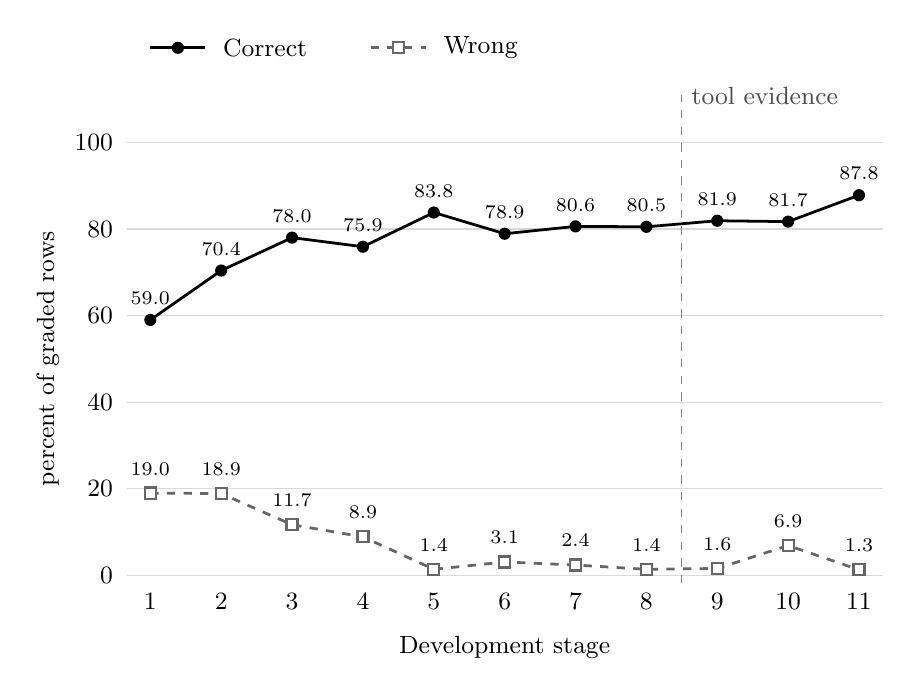
\begin{tikzpicture}[x=1cm,y=1cm,font=\small]
  \foreach \p in {0,20,40,60,80,100} {
    \draw[black!15] (-0.3,{0.055*\p}) -- (9.3,{0.055*\p});
    \node[left] at (-0.35,{0.055*\p}) {\p};
  }
  \foreach \s in {1,...,11} {
    \node[below] at ({(\s-1)*0.9},-0.1) {\s};
  }
  \node[below] at (4.5,-0.65) {Development stage};
  \node[rotate=90] at (-1.3,2.75) {percent of graded rows};
  % judges see tool output from stage 9 on
  \draw[black!50,dashed] (6.75,-0.1) -- (6.75,6.1);
  \node[anchor=south west,black!70] at (6.75,5.85) {tool evidence};
  % correct
  \draw[line width=1pt]
    (0,{0.055*59.0}) -- (0.9,{0.055*70.4}) -- (1.8,{0.055*78.0}) -- (2.7,{0.055*75.9})
    -- (3.6,{0.055*83.8}) -- (4.5,{0.055*78.9}) -- (5.4,{0.055*80.6}) -- (6.3,{0.055*80.5})
    -- (7.2,{0.055*81.9}) -- (8.1,{0.055*81.7}) -- (9.0,{0.055*87.8});
  \foreach \s/\c in {1/59.0,2/70.4,3/78.0,4/75.9,5/83.8,6/78.9,7/80.6,8/80.5,9/81.9,10/81.7,11/87.8} {
    \fill ({(\s-1)*0.9},{0.055*\c}) circle (2.2pt);
    \node[above=2pt] at ({(\s-1)*0.9},{0.055*\c}) {\scriptsize\c};
  }
  % wrong
  \draw[black!60,dashed,line width=1pt]
    (0,{0.055*19.0}) -- (0.9,{0.055*18.9}) -- (1.8,{0.055*11.7}) -- (2.7,{0.055*8.9})
    -- (3.6,{0.055*1.4}) -- (4.5,{0.055*3.1}) -- (5.4,{0.055*2.4}) -- (6.3,{0.055*1.4})
    -- (7.2,{0.055*1.6}) -- (8.1,{0.055*6.9}) -- (9.0,{0.055*1.3});
  \foreach \s/\w in {1/19.0,2/18.9,3/11.7,4/8.9,5/1.4,6/3.1,7/2.4,8/1.4,9/1.6,10/6.9,11/1.3} {
    \fill[white,draw=black!60,line width=.8pt] ({(\s-1)*0.9-0.07},{0.055*\w-0.07}) rectangle ++(0.14,0.14);
    \node[above=3pt] at ({(\s-1)*0.9},{0.055*\w}) {\scriptsize\w};
  }
  % legend
  \draw[line width=1pt] (0,6.7) -- (0.7,6.7);
  \fill (0.35,6.7) circle (2.2pt);
  \node[right] at (0.8,6.7) {Correct};
  \draw[black!60,dashed,line width=1pt] (2.8,6.7) -- (3.5,6.7);
  \fill[white,draw=black!60,line width=.8pt] (3.08,6.63) rectangle ++(0.14,0.14);
  \node[right] at (3.6,6.7) {Wrong};
\end{tikzpicture}
\caption[Correct and wrong percentages of graded rows at the eleven development stages on the 334 tuned emails]{Correct and wrong percentages of graded rows at the eleven development stages on the 334 tuned emails. The dashed vertical line marks the first stage whose grading included tool output. Grading rules and evidence changed along the way, so the stages are comparable only in direction, and none of the stages is a clean measurement. The full table, with the \textsc{Gap} shares and the state of the system at each stage, is Table~\ref{tab:live-history}.}
\label{fig:live-stages}
\end{figure}
